\documentclass[a4paper]{article}

\usepackage{amsmath}
\usepackage{amssymb}
\usepackage{amsfonts}
\usepackage[style=iso]{datetime2}
\usepackage[explicit]{titlesec}
\usepackage{amsthm}
\usepackage{mathrsfs}
\usepackage{array}
\usepackage{graphicx}
\usepackage{mathtools} % Provides \mathrlap command
\usepackage{float}
\usepackage[skip=1em,indent]{parskip}
\usepackage{caption}
\usepackage[hidelinks]{hyperref}
\usepackage{tocloft}
\usepackage{mathtools}

\usepackage{tikz}
\tikzset{>=latex} % for LaTeX arrow head
\usepackage{pgfplots} % for the axis environment
\usetikzlibrary{calc,decorations.markings}

\pgfplotsset{compat=1.18, every tick label/.append style={font=\footnotesize}}

\graphicspath{ {./Images/} }

\makeatletter
\def\th@plain{%
  \thm@notefont{}% same as heading font
  \itshape % body font
}
\def\th@definition{%
  \thm@notefont{}% same as heading font
  \normalfont % body font
}
\makeatother

\newcommand*\diff{\mathop{}\!d} % for the differential in integrals

% ---------------- %
\newcommand{\R}{\mathbb{R}}
\newcommand{\C}{\mathbb{C}}

\NewCommandCopy{\oldIm}{\Im}
\renewcommand{\Im}{\mathop{\oldIm\mathfrak{m}}}
\NewCommandCopy{\oldRe}{\Re}
\renewcommand{\Re}{\mathop{\oldRe\mathfrak{e}}}

\newcommand{\overbar}[1]{\mkern 1.5mu\overline{\mkern-1.5mu#1\mkern-1.5mu}\mkern 1.5mu}
% ---------------- %

\newtheorem{theorem}{Theorem}
\newtheorem{lemma}[theorem]{Lemma}
\newtheorem{proposition}[theorem]{Proposition}
\newtheorem{corollary}{Corollary}[theorem]

\theoremstyle{definition}
\newtheorem{definition}{Definition}

% \setlength{\cftsecnumwidth}{3em}

\begin{titlepage}
\title{P\'olya Vector Fields}
\author{Abdul Musthakin}
\date{\today}
\end{titlepage}

% \renewcommand{\thesection}{\Roman{section}}

\allowdisplaybreaks

\setlength{\parindent}{0pt}

\begin{document}
\maketitle

\section{Introduction}

Let $X \subseteq \C$.
Consider some arbitrary complex function $f \colon X \to \C$ defined by $z \mapsto f(z)$.
We can define $u,v \colon X \to \R$ by $u(z) \coloneq \Re f (z)$ and $v(z) \coloneq \Im f(z)$.
Then, $f(z) = u(z) + i v(z)$.
We may use $f = u + i v$ as shorthand for this, and omitting the arguments of such functions will be done when context removes ambiguity.

In general, we may associate $\mathbb{C}$ with $\R^2$ via the bijection $\phi \colon \C \to \R^2$ given by $\phi(z) \coloneq (\Re z, \Im z)$.
The inverse is simply $\phi^{-1} \colon \R^2 \to \C$ given by $\phi^{-1}(x,y) = x + iy$.
Then, the map $\phi[X] \to \C$, $(x,y) \mapsto f\left(\phi^{-1}(x,y)\right)$ may be associated with the complex function $f$, and likewise for $u$ and $v$.
It then makes sense to refer to $f(x,y)$ and similar expressions.
Note that this association gives us $z \coloneq x + iy$ for arbitrary $x,y,z$ in their respective sets.

Furthermore, we may define the vector field $\mathbf{H} \colon \phi[X] \to \R^2$ by $\mathbf{H}(x,y) \coloneq \phi^{-1} (f(x,y))$.
It follows that $\mathbf{H} = u\mathbf{\hat{x}} + v\mathbf{\hat{y}}$.
Plotting vector fields is something that we can do, so we now have a way to visualise complex functions.
As plotting the vector field with the normal lengths of the vectors would result in something very cluttered, we can normalise it.
\begin{equation*}
    \mathbf{\hat{H}} \coloneq \frac{\mathbf{H}}{\lvert \mathbf{H} \rvert}
\end{equation*}
Every time we refer to plotting a vector field, this will be what we actually plot.
In order to reintroduce the information of the vector's magnitudes, we can use colour.
A simple colour bar will accompany our figures.

Now, let us consider a concrete example with $f \colon \C \to \C$ given by $f(z) \coloneq z$.
We thus have $\mathbf{H} = x\mathbf{\hat{x}} + y\mathbf{\hat{y}}$.
Since
\begin{equation*}
    \lvert f(z) \rvert = \lvert z \rvert = \sqrt{x^2 + y^2},
\end{equation*}
we have
\begin{equation*}
    \mathbf{\hat{H}} \coloneq \frac{\mathbf{H}}{\lvert \mathbf{H} \rvert} = \frac{1}{\sqrt{x^2+y^2}} \mathbf{\hat{x}} + \frac{y}{\sqrt{x^2+y^2}} \mathbf{\hat{y}}.
\end{equation*}
The vector field $\mathbf{\hat{H}}$ has been plotted below.
\begin{figure}[H]
    \centering
    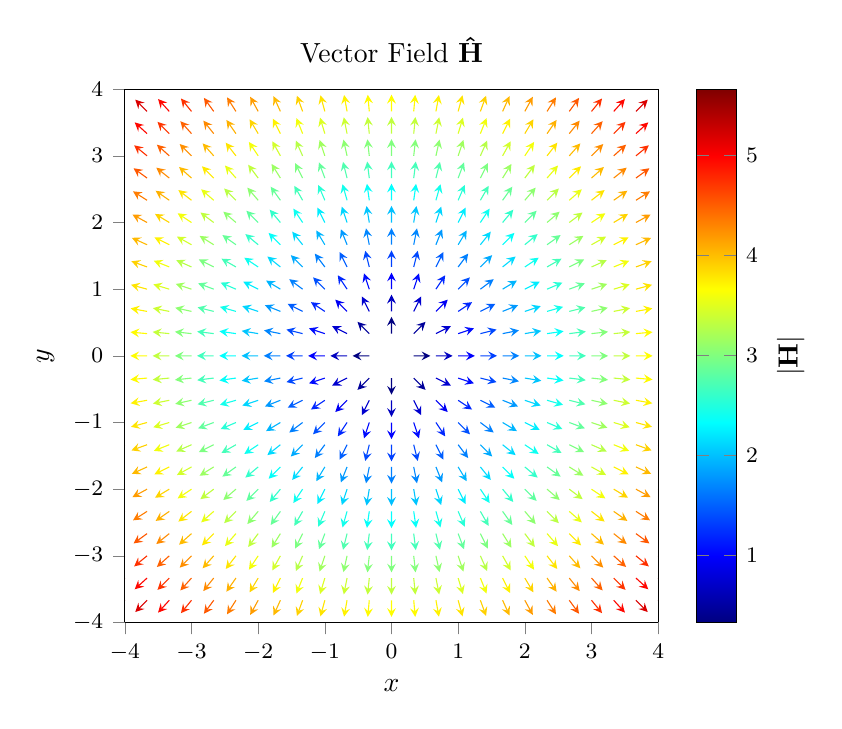
\begin{tikzpicture}
        \begin{axis}[
                xmin = -4, xmax = 4,
                ymin = -4, ymax = 4,
                zmin = 0, zmax = 1,
                axis equal image,
                xtick distance = 1,
                ytick distance = 1,
                tick align = outside,
                xtick pos= left,
                ytick pos= left,
                view = {0}{90},
                scale = 1.25,
                title = {Vector Field $\mathbf{\hat{H}}$},
                height=7cm,
                xlabel = {$x$},
                ylabel = {$y$},
                colormap/jet,
                colorbar,
                colorbar style = {
                        ylabel = {$\lvert \mathbf{H} \rvert$}
                    },
            ]
            \addplot3[
                point meta = {sqrt(x^2+y^2)},
                quiver = {
                        u = {x/sqrt(x^2+y^2)},
                        v = {y/sqrt(x^2+y^2)},
                        scale arrows = 0.25,
                    },
                quiver/colored = {mapped color},
                -stealth,
                domain = -4:4,
                domain y = -4:4,
                restrict expr to domain={sqrt(x^2+y^2)}{0.01:100},
            ] {0};
        \end{axis}
    \end{tikzpicture}
\end{figure}

\section{P\'olya Vector Fields}

Our previous visualisation was fine, as it gave us an idea of the function's behaviour within the subset of the domain that was chosen.
The vector field has reflectional and rotational symmetry about the origin, but is this a meaningful observation?
Certainly, with functions $\R \to \R$, such symmetries can lead to analytical properties.
For example, even and odd functions exhibit symmetry, which leads to the following results (assuming integrability).
\begin{align*}
     & f \colon \R \to \R \text{ is odd} \leadsto \int_{-A}^{A} f(x) \diff x = 0                            \\
     & f \colon \R \to \R \text{ is even} \leadsto \int_{-A}^{A} f(x) \diff x = 2 \int_{0}^{A} f(x) \diff x
\end{align*}
More generally, we can get a good idea of the sign of an integral from the graph of a function.
That does not seem to translate well to complex functions.
Suppose we wish to evaluate the integral of $f(z) \coloneq z$ along some closed contour $C$.
The function is holomorphic and entire
Therefore, by \textbf{Cauchy's theorem},
\begin{equation*}
    \oint_C f(z) \diff z = 0.
\end{equation*}
Could we have figured that out, or at least have obtained an idea of what it would be, from the graph above?
Sure, our visualisation of $f$ is symmetric about the origin under rotations or reflections, but the above result holds under any closed contour -- which might not even include the origin.
This is why we will introduce a specific type of vector field, which we can interpret in a meaningful way for the purpose of integration.
\begin{definition}[P\'olya Vector Field]
    Let $X \subseteq \C$, and let $f,u,v \colon X \to \C$ such that $u \coloneq \Re f$ and $v \coloneq \Im f$.
    The P\'olya vector field of $f$, $\mathbf{\overbar{H}} \colon \phi[X] \to \R^2$, is given by $\mathbf{\overbar{H}} (x,y) \coloneq \phi^{-1}(\overbar{f(x,y)})$.
    Equivalently, $\mathbf{\overbar{H}} \coloneq u\mathbf{\hat{x}} - v\mathbf{\hat{y}}$.
\end{definition}
The P\'olya vector field of $f$ is the vector field associated with its conjugate, which, in our case, is given by
\begin{equation*}
    \overbar{f(z)} = \overbar{z} = x - iy.
\end{equation*}
Thus, we have $\mathbf{\overbar{H}} \colon \R^2 \to \R^2$ given by
\begin{equation*}
    \mathbf{\overbar{H}}(x,y) = x \mathbf{\hat{x}} - y \mathbf{\hat{y}}.
\end{equation*}
Plotting this gives the following graph.
\begin{figure}[H]
    \centering
    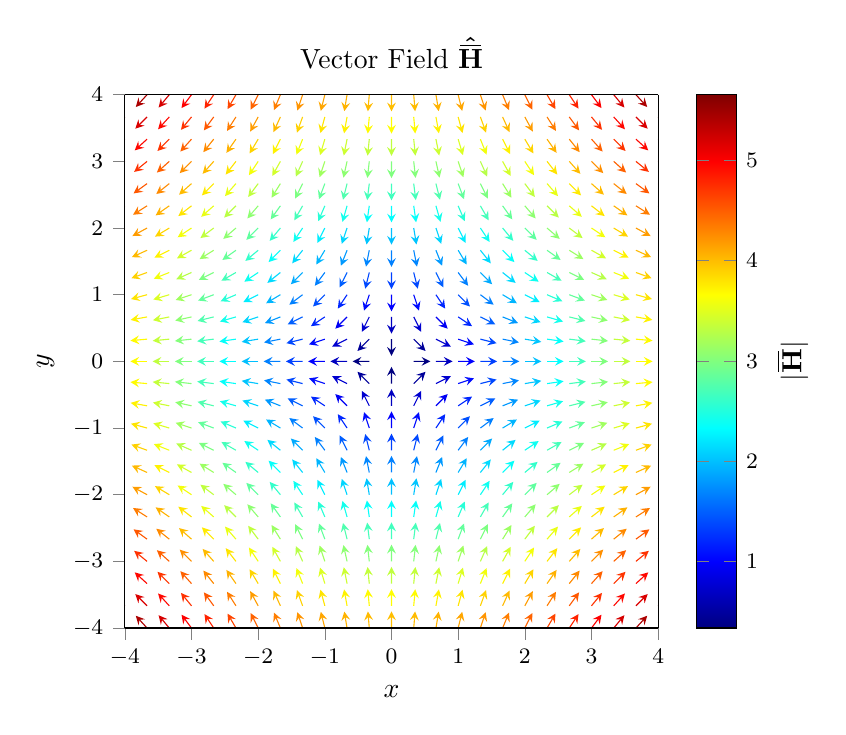
\begin{tikzpicture}
        \begin{axis}[
                xmin = -4, xmax = 4,
                ymin = -4, ymax = 4,
                zmin = 0, zmax = 1,
                axis equal image,
                xtick distance = 1,
                ytick distance = 1,
                tick align = outside,
                xtick pos= left,
                ytick pos= left,
                view = {0}{90},
                scale = 1.25,
                title = {Vector Field $\mathbf{\hat{\overbar{H}}}$},
                height=7cm,
                xlabel = {$x$},
                ylabel = {$y$},
                colormap/jet,
                colorbar,
                colorbar style = {
                        ylabel = {$\lvert \mathbf{\overbar{H}} \rvert$}
                    },
            ]
            \addplot3[
                point meta = {sqrt(x^2+y^2)},
                quiver = {
                        u = {x/sqrt(x^2+y^2)},
                        v = {-y/sqrt(x^2+y^2)},
                        scale arrows = 0.25,
                    },
                quiver/colored = {mapped color},
                -stealth,
                domain = -4:4,
                domain y = -4:4,
                restrict expr to domain={sqrt(x^2+y^2)}{0.01:100},
            ] {0};
        \end{axis}
    \end{tikzpicture}
\end{figure}
Why is this any better?
To answer that, let us rewrite the integral we had before, using the arbitrary parameterisation $z \colon \C \to \C$, $x,y \colon \R \to \R$, $z(t) \coloneq x(t) + iy(t)$ with $t \in [a,b]$.
Henceforth, we need not consider any specific complex function.
\begin{align*}
    \oint_C f(z) \diff z \coloneq & \int_a^b f(z(t)) z'(t) \diff t                                                                                                                          \\
    =                             & \int_a^b [u(z(t)) + i v(z(t))] [x'(t) + i y'(t)] \diff t                                                                                                \\
    =                             & \int_a^b [u(z(t))x'(t) - v(z(t))y'(t)] \diff t                                                                                                          \\
    \phantom{=}                   & + i \int_a^b [u(z(t))y'(t) + v(z(t))x'(t)] \diff t                                                                                                      \\
    =                             & \int_a^b [u(x(t) + i y(t))x'(t) - v(x(t) + i y(t))y'(t)] \diff t                                                                                        \\
    \phantom{=}                   & + i \int_a^b [u(x(t) + i y(t))y'(t) + v(x(t) + i y(t))x'(t)] \diff t                                                                                    \\
    =                             & \int_a^b [u(x(t), y(t))x'(t) - v(x(t), y(t))y'(t)] \diff t                                                                                              \\
    \phantom{=}                   & + i \int_a^b [u(x(t), y(t))y'(t) + v(x(t), y(t))x'(t)] \diff t                                                                                          \\
    =                             & \int_a^b \mathbf{\overbar{H}}(x(t), y(t)) \cdot \mathbf{r}'(t) \diff t + i \int_a^b \mathbf{\overbar{H}}(x(t), y(t)) \cdot \mathbf{r}_\perp'(t) \diff t \\
    =                             & \oint_C \mathbf{\overbar{H}} \cdot \mathbf{\hat{T}} \diff s + i \oint_C \mathbf{\overbar{H}} \cdot \mathbf{\hat{N}} \diff s
\end{align*}
Even this, involving the proper definition of the contour integral being applied, is not without omission of details.
It must be said that we have overloaded the symbol $C$ with both a curve in $\C$ and a corresponding curve in $\R^2$.
A less direct derivation of the same result is as follows.
\begin{align*}
    \oint_C f(z) \diff z & = \oint_C (u + iv) (\diff x + i \diff y)                                                                                      \\
                         & = \oint_C (u \diff x - v \diff y) + i \oint_C (u \diff y + v \diff x)                                                         \\
                         & = \oint_C \mathbf{\overbar{H}} \cdot \mathbf{\hat{T}} \diff s + i \oint_C \mathbf{\overbar{H}} \cdot \mathbf{\hat{N}} \diff s
\end{align*}
This may be considered abuse of notation without further definitions and clarification.
Regardless, we have shown that P\'olya vector fields allow us to write any (closed) contour integral as a work and flux integral.
\begin{equation} \label{eq:work-flux}
    \oint_C f(z) \diff z = \mathfrak{W}[\mathbf{\overbar{H}}, C] + i \mathfrak{F}[\mathbf{\overbar{H}}, C]
\end{equation}
That alone is an aesthetically pleasing result, though there is further utility.
Consider the surface $S$ such that $\partial S \coloneq C$.
Then, by \textbf{Green's theorem},
\begin{equation*}
    \mathfrak{W}[\mathbf{\overbar{H}}, C] = \iint_S \nabla \times \mathbf{\overbar{H}}.
\end{equation*}
By the \textbf{divergence theorem} in two dimensions, which is equivalent to Green's theorem,
\begin{equation*}
    \mathfrak{F}[\mathbf{\overbar{H}}, C] = \iint_S \nabla \cdot \mathbf{\overbar{H}}.
\end{equation*}
Therefore,
\begin{equation}
    \oint_C f(z) \diff z = \iint_S \nabla \times \mathbf{\overbar{H}} + i \iint_S \nabla \cdot \mathbf{\overbar{H}}.
\end{equation}
This is the insightful result we were after, which is seen by the fact that Cauchy's theorem follows almost immediately afterwards.

\section{Cauchy's Theorem}

If $f$ is holomorphic, then $u$ and $v$ satisfy the \textbf{Cauchy-Riemann equations}.
\begin{align*}
    \partial_x u & = \partial_y v  \\
    \partial_y u & = -\partial_x v
\end{align*}
However, one can write the divergence and curl of $\mathbf{\overbar{H}}$ explcitly as follows.
\begin{align*}
    \nabla \cdot \mathbf{\overbar{H}}  & = \partial_x u - \partial_y v \\
    \nabla \times \mathbf{\overbar{H}} & = \partial_x v + \partial_y u
\end{align*}
It can thus be seen that $f$ being holomorphic implies that $\nabla \cdot \mathbf{\overbar{H}} = \nabla \times \mathbf{\overbar{H}} = 0$.
Therefore,
\begin{equation}
    \oint_C f(z) \diff z = 0,
\end{equation}
no matter what the closed contour $C$ actual is, showing that our result is path independent.

This is not a proof of the theorem, and an actual proof would preferably not use Green's theorem.
This is because it would then have to assume that the partial derivatives of $u$ and $v$ are continuous -- not strictly a requirement, but considerably more work would need to be done otherwise.
Additionally, the condition of $X$ being simply connected has not been discussed, nor any of the subtleties regarding the validity of Green's theorem in this scenario.

Our goal is not to prove Cauchy's theorem and other results in complex analysis using P\'olya vector fields, but rather to provide an alternative lens to view them in and gain intuition.
We have shown that the holomorphicity of $f$ is directly related to the properties of $\mathbf{\overbar{H}}$.
A complex function is holomorphic iff its P\'olya vector field is irrotational and incompressible.
That is a beautiful result.

Moreover, we may obtain useful information from $\mathbf{\overbar{H}}$ in other situations.
None of the steps involved in the derivation of Equation~\eqref{eq:work-flux} required $C$ to be a closed contour.
That means that we have a much more general result.
By observing how $\mathbf{\overbar{H}}$ appears to flow through and across a contour, we can estimate the value of the integral along the contour.

\section{Meromorphic Functions}

A complex function $f \colon X \to \C$ is meromorphic on $D \subseteq \C$ iff it is holomorphic on $D$ except for a set of poles of $f$.
For example, the function $f \colon \C \setminus \{0\} \to \C$ defined by
\begin{equation*}
    f(z) \coloneq \frac{1}{z} = \frac{\bar{z}}{z\bar{z}} = \frac{\bar{z}}{\lvert z \rvert^2} = \frac{x - iy}{x^2 + y^2},
\end{equation*}
is meromorphic on $\C$.
We also have
\begin{equation*}
    u(z) = \frac{x}{x^2+y^2},
\end{equation*}
and
\begin{equation*}
    v(z) = -\frac{y}{x^2+y^2}.
\end{equation*}
Additionally, the magnitude of $f(z)$ is given by
\begin{equation*}
    \lvert f(z) \rvert = \left\lvert \frac{\bar{z}}{\lvert z \rvert^2} \right\rvert = \frac{\lvert \bar{z} \rvert}{\lvert z \rvert^2} = \frac{1}{\lvert z \rvert} = \frac{1}{\sqrt{x^2+y^2}}.
\end{equation*}
Since
\begin{equation*}
    \overline{f(z)} = \frac{x+iy}{x^2+y^2},
\end{equation*}
the P\'olya vector field of $f$, $\mathbf{\overbar{H}} \colon \R^2 \setminus \{(0,0)\}$, is given by
\begin{equation*}
    \mathbf{\overbar{H}}(x,y) = \frac{x}{x^2+y^2} \mathbf{\hat{x}} + \frac{y}{x^2+y^2} \mathbf{\hat{y}}.
\end{equation*}
We have used a logarithmic scale for the colour bar instead of the regular one to more evenly distribute the colours.
Plotting $\mathbf{\overbar{H}}$ gives the following graph.
\begin{figure}[H]
    \centering
    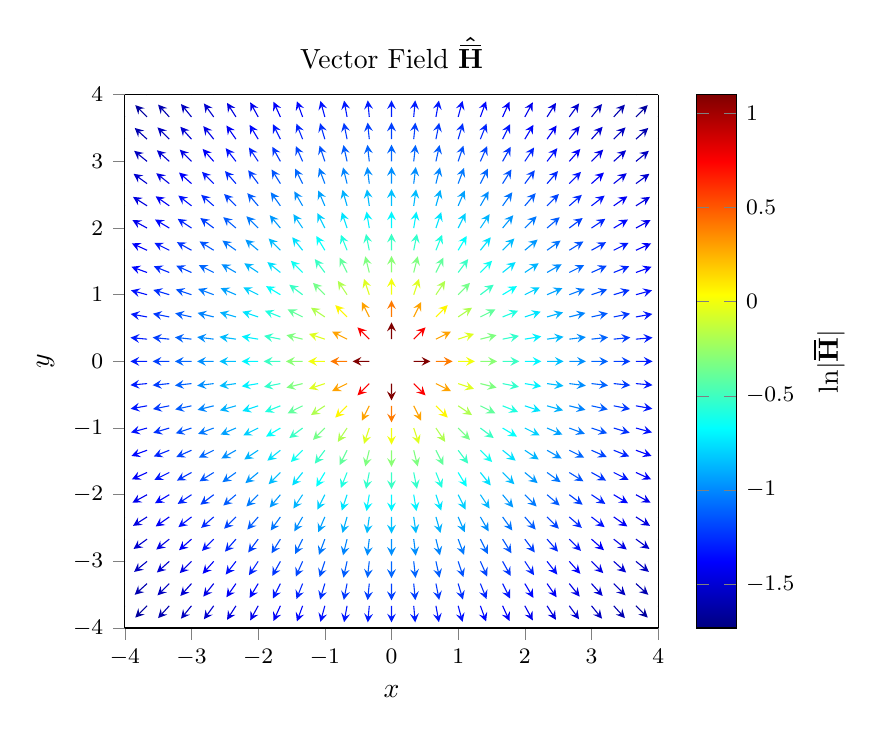
\begin{tikzpicture}
        \begin{axis}[
                xmin = -4, xmax = 4,
                ymin = -4, ymax = 4,
                zmin = 0, zmax = 1,
                axis equal image,
                xtick distance = 1,
                ytick distance = 1,
                tick align = outside,
                xtick pos= left,
                ytick pos= left,
                view = {0}{90},
                scale = 1.25,
                title = {Vector Field $\mathbf{\hat{\overbar{H}}}$},
                height=7cm,
                xlabel = {$x$},
                ylabel = {$y$},
                colormap/jet,
                colorbar,
                colorbar style = {
                        ylabel = {$\ln \lvert \mathbf{\overbar{H}} \rvert$}
                    },
            ]
            \addplot3[
                point meta = {ln(1/sqrt(x^2+y^2))},
                quiver = {
                        u = {(x/(x^2+y^2))*sqrt(x^2+y^2)},
                        v = {(y/(x^2+y^2))*sqrt(x^2+y^2)},
                        scale arrows = 0.25,
                    },
                quiver/colored = {mapped color},
                -stealth,
                domain = -4:4,
                domain y = -4:4,
                restrict expr to domain={sqrt(x^2+y^2)}{0.01:100},
            ] {0};
        \end{axis}
    \end{tikzpicture}
\end{figure}
The most obvious feature of this vector field is the `source' at the origin.
However, it would not make sense to comment about $\nabla \cdot \mathbf{\overbar{H}}$ at $(0,0)$, because $\mathbf{\overbar{H}}$ is not defined at that point.
Everywhere that $\mathbf{\overbar{H}}$ is defined, it is irrotational and incompressible, follows from the holomorphicity of $f$.
Therefore, any integral along a contour that does not enclose the origin will evaluate to zero.

What if it does enclose the origin?
Suppose we wish to evaluate the integral of $f$ along the anticlockwise unit circle.
Let us call this contour $\gamma$.
We can parameterise $\gamma$ by $z(t) \coloneq e^{it}$ with $t \in [0, 2\pi]$.
Then, $z'(t) = ie^{it} = iz(t)$.
Our contour integral is given by
\begin{align*}
    \oint_\gamma f(z) \diff z & = \oint_\gamma \frac{\diff z}{z}           \\
                              & = \int_0^{2\pi} \frac{z'(t)}{z(t)} \diff t \\
                              & = \int_0^{2\pi} \frac{iz(t)}{z(t)} \diff t \\
                              & = i \int_0^{2\pi} \diff t                  \\
                              & = 2\pi i.
\end{align*}
This is interesting.
Despite the fact the P\'olya vector field of $f$ has properties very similar to the previous one we discussed, we have obtained a completely different result.
Whilst $f$ is holomorphic everywhere it is defined, $\C \setminus \{0\}$ is not simply connected.
Informally, this means that we cannot shrink any loop (that originally surrounds the origin) down to single point without touching the origin.
Without our domain being simply connected, we cannot apply Cauchy's theorem.

It is is not the case that we are dealing with a function which is not holomorphic, such as $g \colon \C \to \C$ given by $g(z) \coloneq \lvert z \rvert$.
The P\'olya vector field of $g$ has zero curl, but nonzero divergence.
Our function $f$ is holomorphic, but the hole in its domain breaks the `rule' we had and leads to unusual results.
This idea, in its general sense, is further studied in higher-level mathematics.

Since the contour integral evaluated to a purely imaginary number, we know that only the flux integral contributed to it.
That makes sense, if you imagine the unit circle on the vector field plot above.
The field lines are entirely perpendicular to the contour, so there is zero work.
The lines flow out of the circle, from the source at the origin, so there is positive flux.
\begin{align*}
    \mathfrak{W}[\mathbf{\overbar{H}}, C] & = 0    \\
    \mathfrak{F}[\mathbf{\overbar{H}}, C] & = 2\pi
\end{align*}
We did not need to choose the unit circle as our contour.
As $f$ is holomorphic everywhere it is defined, we can deform the contour into a circle of any radius, or any other contour.
As long as it encloses the origin, the integral will evaluate to the same number.
\end{document}